\selectlanguage{ngerman}%
\frenchspacing%
\begin{ledgroupsized}[r]{120mm}%
\footnotesize%
\pstart%
\noindent\textbf{Überlieferung:}%
\pend%
\end{ledgroupsized}%
\begin{ledgroupsized}[r]{114mm}%
\footnotesize%
\pstart%
\parindent -6mm%
\makebox[6mm][l]{\textit{L}}%
Aufzeichnung:
LH~XXXV~11,\;14 Bl.\;34.
Ein Zettel (etwa 6\;x\;8~cm),
Ränder beschnitten.
Zwei Seiten.
\pend
\end{ledgroupsized}
\vspace{5mm}%
\begin{ledgroup}%
\footnotesize%
\pstart%
\noindent%
\textbf{Datierungsgründe:}
Die Datierung der Aufzeichnung N.\;\ref{58949} beruht %
auf inhaltlichen Betrachtungen.
Siehe die ausführliche Begründung auf S.\;\pageref{58949_dat}.
\pend%
\end{ledgroup}%
\selectlanguage{latin}%
\frenchspacing%
\vspace{6mm}%
\pstart%
\normalsize%
\noindent%
\lbrack%
\href{\Scan{LH_35_11_14_034r}}%
{34\,r\textsuperscript{o}}%
\rbrack%
\pend%
\vspace{-1.0em}
\centerline{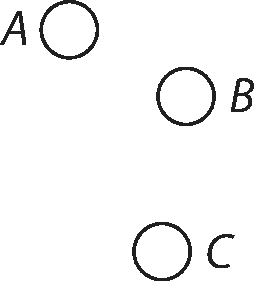
\includegraphics[width=0.145\textwidth]{gesamttex/edit_VIII-4/images/LH_35_11_14_034_d_034r.pdf}}
\nobreak\vspace{0.5em}
\centerline{\lbrack\textit{Fig.\:1}\rbrack}
\vspace{1.25em}
\pstart%
\noindent%
\edlabel{LH_35_11_14_034_034rv_drstllng-1}%
Si trium corporum \textit{A}, \textit{B}, \textit{C}%
\indexS{corpora concurrentia}
ponatur motus quicunque%
\indexS{motus quicunque}
et demto motu communi%
\indexS{motus communis demtus}
qui est communis centri gravitatis,%
\indexS{centrum gravitatis commune}%
\indexS{motus centri gravitatis}
cuique assignetur motus proprius,%
\indexS{motus proprius}
atque inde quaeratur vis respectiva%
\indexS{vis respectiva quaesita}%
\lbrack,\rbrack\ 
quae tribus modis inveniri potest,%
\indexS{modus inveniendi vim respectivam}
quaerendo eam inter \textit{A} et $B+C,$
inter \textit{B} et $A+C$,
inter \textit{C} et 
\edtext{%
$A+B,$ et%
}{%
\lemma{$A+B,$}%
\Bfootnote{%
\textit{(1)}~inter %
\textit{(2)}~et%
~\textit{L}%
}}
debet semper provenire
\edlabel{LH_35_11_14_034_034r_gfrs-1}%
idem.%
\edtext{}{%
\xxref{LH_35_11_14_034_034r_gfrs-1}{LH_35_11_14_034_034r_gfrs-2}%
\lemma{idem.}\Bfootnote{%
\textit{(1)}~Sufficitque
\textit{(2)}~Hac methodo determinari poterit%
~\textit{L}}}
Hac methodo determinari poterit%
\indexS{methodus inveniendi vim respectivam}%
\edlabel{LH_35_11_14_034_034r_gfrs-2}
\lbrack%
\href{\Scan{LH_35_11_14_034v}}%
{34\,v\textsuperscript{o}}%
\rbrack%
quid post concursum corporum%
\indexS{concursus corporum}
(\protect\vphantom)%
demto communi motu centri gravitatis,%
\indexS{motus communis centri gravitatis}%
\indexS{motus communis demtus}
\edtext{%
qui perdurat%
\protect\vphantom()%
}{%
\lemma{qui}\Bfootnote{%
perdurat
\textit{erg.\;L}}}
fieri debeat.
\edlabel{LH_35_11_14_034_034v_hypoth-1}%
Utcunque enim corpora colligari ponas,%
\indexS{corpora colligata}
semper debet servari in summa%
\indexS{summa potentiae respectivae}
eadem quantitas potentiae respectivae.%
\indexS{potentia respectiva servanda}%
\indexS{quantitas potentiae respectivae}%
\edlabel{LH_35_11_14_034_034v_hypoth-2}%
\edlabel{LH_35_11_14_034_034rv_drstllng-2}
Quid si singula
\edtext{%
corpora singulis%
}{%
\lemma{corpora}\Bfootnote{\hspace{-0,75mm}%
\bars{lineis rectis colliges tendibilibus et comprimilibus et \textit{gestr.}}
singulis%
~\textit{L}}}
compares,
an licebit sic
\edtext{\lbrack quoque\rbrack}{%
\lemma{quotque}\Bfootnote{%
\textit{L~ändert Hrsg.}}}
aestimare vim respectivam?%
\indexS{vis respectiva aestimanda}
Sed optimum erit sic progredi,
ut duorum aestimetur vis respectiva%
\indexS{vis respectiva aestimanda}
inter se,
et deinde centri gravitatis%
\indexS{centrum gravitatis commune}
eorum cum tertio.
\edlabel{LH_35_11_14_034_034v_proexc-1}%
Haec methodus%
\indexS{methodus pro concursu eccentrico}%
\indexS{methodus inveniendi vim respectivam}
etiam pro concursu eccentrico%
\indexS{concursus eccentricus}%
\lbrack,\rbrack\
ponendo corpus excipiens%
\indexS{corpus excipiens divisum}
divisum in duas partes%
\lbrack,\rbrack\
unam
quae maxima incursus centrici%
\indexS{incursus centricus}
assumi potest,
alteram
quae eccentrice excipit.%
\edlabel{LH_35_11_14_034_034v_proexc-2}
\edlabel{LH_35_11_14_034_034v_cntrgyr-1}%
Unde cum fit gyrus%
\indexS{gyrus}
simul et progressus%
\indexS{progressus in concursu eccentrico}%
\lbrack,\rbrack\
corpora gyrantur%
\indexS{corpus gyrans}
circa idem
\edtext{%
centrum%
\indexS{centrum gyrationis}
quod%
}{%
\lemma{centrum}%
\Bfootnote{%
\textit{(1)}~in %
\textit{(2)}~ad
\textit{(3)}~quod %
\textit{L}%
}}
est eorum centr. gr.%
\indexS{centrum gravitatis commune}%
\edlabel{LH_35_11_14_034_034v_cntrgyr-2}
Habent et vim respectivam%
\indexS{vis respectiva aestimanda}
quae quadratum est gyri%
\indexS{gyrus}
in corpus.%
\indexS{quadratum gyri in corpus}%
\textls{ Comprobatio seu examen,}%
\indexS{comprobatio}%
\indexS{examen}
si effici possit altero concursu%
\indexS{concursus alter}
restitutio in statum priorem.%
\indexS{status prior}%
\indexS{restitutio in statum priorem}%
\pend%
\newpage%
\pstart%
\noindent%
\centering%
*     *     *
\pend%
\selectlanguage{ngerman}%
\frenchspacing%
\vspace{4.0em}%
\begin{ledgroup}%
\footnotesize%
\pstart%
\noindent%
\textls{Ausführliche Datierungsgründe:}%
\pagelabel{58949_dat}
Der Träger der titellosen und undatierten Aufzeichnung N.\;\ref{58949} weist weder Spuren eines Wasserzeichens noch sonstige äußere Merkmale, die eine eindeutige Datierung ermöglichen würden.
Aus inhaltlichen Gründen erweist sich eine grobe chronologische Einordnung des Textes dennoch als möglich.
\pend%
\pstart%
Die in der Aufzeichnung N.\;\ref{58949} dargelegte Methode zur Bestimmung der Kinematik dreier zusammenstoßender Körper wird ausführlich in dem von Leibniz eigenhändig auf den 31.\;Oktober\,/\,10. November 1690 datierten Entwurf N.\;\ref{58939} \textit{Scheda secunda de impulsu eccentrico} angewandt.
Beide Texte gehen von derselben Voraussetzung aus:
Ungeachtet, wie man die einzelnen Körper untereinander gruppiert, \textit{semper debet servari in summa eadem quantitas potentiae respectivae} (\refpassage{LH_35_11_14_034_034v_hypoth-1}{LH_35_11_14_034_034v_hypoth-2}; vgl. \refpassage{LH_35_11_14_003-004_004v_methodus-1}{LH_35_11_14_003-004_004v_methodus-2}).
Dass die Aufzeichnung N.\;\ref{58949} besonders die Anwendbarkeit dieser Methode auf den exzentrischen Stoß hervorhebt (\refpassage{LH_35_11_14_034_034v_proexc-1}{LH_35_11_14_034_034v_proexc-2}), ist Grund für die Vermutung einer gemeinsamen Abfassungszeit mit der \textit{Scheda secunda}: %
N.\;\ref{58949} könnte entweder als Verallgemeinerung der in N.\;\ref{58939} erzielten Ergebnisse entstanden sein, oder aber als Skizze, durch welche die Untersuchung in N.\;\ref{58939} angespornt worden sein könnte.
Unter dieser Annahme ergibt sich als wahrscheinliche Abfassungszeit der Aufzeichnung N.\;\ref{58949} der Herbst 1690. %
Eine frühere oder eine spätere Datierung sind allerdings möglich.
\pend%
\pstart%
Eine Entstehung der Aufzeichnung N.\;\ref{58949} vor der auf den Zeitraum von April bis spätestens Oktober 1690 datierbaren Aufzeichnung N.\;\ref{60300} ist jedoch aus folgendem Grund auszuschließen:
In der Aufzeichnung N.\;\ref{58949} wird unvermittelt angenommen, dass beim exzentrischen Stoß eine Drehung entstehe, deren Zentrum %
mit dem Schwerpunkt des gestoßenen Körpers zusammenfalle (\refpassage{LH_35_11_14_034_034v_cntrgyr-1}{LH_35_11_14_034_034v_cntrgyr-2}).
Folglich muss N.\;\ref{58949} nach der %
Aufzeichnung N.\;\ref{60300} abgefasst worden sein.
Denn erst in N.\;\ref{60300} berichtigt Leibniz seine frühere (etwa in N.\;\ref{impulsuseccentricus} %
vertretene) Ansicht, das Zentrum der Drehung beim exzentrischen Stoß falle mit dem Schwerpunkt des indirekt angestoßenen Teils des Körpers zusammen (vgl. N.\;\ref{60300}, \refpassage{LH_37_05_044_044r_cntrgyr-1}{LH_37_05_044_044r_cntrgyr-2}; siehe auch die Datierungsgründe, S.\;\pageref{LH_37_05_044_datierung}).
Wenn damit -- wenigstens im Hinblick auf die relative Chronologie -- ein Terminus post quem ermittelbar ist, lässt sich hingegen kein klarer Terminus ante quem der Datierung von N.\;\ref{58949} zum Redaktionsschluss angeben.%
\pend%
\pstart%
Schließlich sei erwähnt, dass der letzte Satz der Aufzeichnung N.\;\ref{58949} (\textit{Comprobatio seu examen, si effici possit altero concursu restitutio in statum priorem}) eine Anwendung der Methode vorschlägt, die Leibniz bereits Anfang 1678 in seiner Untersuchung \textit{De corporum concursu} dargestellt hatte;
siehe \textit{LSB} VIII,\;3 N.\;58\textsubscript{2}, S.\;542.15\textendash23.\cite{01401}
\pend%
\end{ledgroup}%
\selectlanguage{latin}%
\frenchspacing%
\normalsize%
